% !TEX encoding = UTF-8 Unicode

\documentclass[twocolumn,10pt,a4j]{ltjsarticle}
\usepackage{kougai}

\title{Webサイトの最適な広告配置方法とテキストによる印象の調査}
\author{1932135 村上 航介  指導教員 須田 宇宙 准教授}
\date{}

\begin{document}

\maketitle

\section{はじめに}
%背景
近年,インターネット市場が年々需要が高まっているなか,広告において,TV・新聞などのマスメディアよりも,検索エンジン,Webサイト,アプリ,SNSなどインターネットを介して利用するメディアやサービスに広告を掲載する企業が増加している.また,インターネット広告自体のテキストのフォントの色使い,大きさなどの印象による宣伝効果への影響については明確になっていない.

%問題点
また,広告の配置によっては,ユーザにとって煩わしい位置にあるWebページが存在し,広告収益によるトレードオフを考えながら配置する必要がある.
これに対して,モバイル端末における広告配置についての研究があり,モバイル端末における有力な広告配置方法が挙げられている\cite{mobile}.
しかし,パソコン上での宣伝効果に適した広告配置が明らかになっていないという問題点があり,また,フォントによる印象についての研究は行われているが,広告におけるフォントに関する研究が行われていないことも問題となっている.

%目的
そこで本研究では,パソコン上における,Webサイトの広告配置とテキストによる煩わしさおよび宣伝効果の違いや影響を調査し,比較することを目的とする.

\section{インターネット広告}
2021年では,インターネット広告費がマスコミ四媒体広告費用(新聞/雑誌/ラジオ/テレビメディアの媒体費と製作費の合算)を上回ったことが報告されている\cite{dentsu}.

また,インターネット広告といっても様々な広告形態が存在し,そのなかでも,検索エンジンやWebサイト,アプリなどの広告枠に表示される画像,動画,テキスト広告のことを「ディスプレイ広告」という.
特徴としては,年齢や性別,過去のWebの閲覧履歴などをもとに,興味を持ってもらいたい層をターゲティングできる点が挙げられ,潜在層から顕在層に向けて幅広く訴求できる傾向にあるので,幅広い広告表現で視覚的に印象が与えられる.
%訴求:消費者の購買意欲に働きかける

\section{実験概要と結果}
本研究では,パソコン上のWebサイトにおける広告の煩わしさと宣伝効果に関して,広告配置と広告のテキストのフォントの影響について調査する.
宣伝効果の指標として,表示されていた広告に関する問題を出題し,その正答率を用いる.
煩わしさの指標として,煩わしさについて4段階で評価してもらい算出する.

広告配置については,広告を画面右部・記事内・記事終わりに配置した記事を作成し使用した.
広告のテキストのフォントについては,フォントをゴシック体・明朝体・丸ゴシックとした記事を作成し使用した.
いずれも被験者が記事を読んだ後に調査を行った.

パソコンで見てもらうのを前提としているので,調査対象はパソコンを使用することが多い大学生を対象とする.
広告配置と広告のテキストのフォントによる調査は別日程で行った.

調査結果を図\ref{fig:結果}に示す.
横軸が宣伝効果,縦軸が煩わしさを表している.
広告配置の調査結果から,記事終わりに置くことが最も煩わしさが低く,宣伝効果が高いことが分かった.
フォントの調査結果から,丸ゴシック体とゴシック体が煩わしさが低く,丸ゴシック体が最も宣伝効果が高いことが分かった.
これらから,煩わしさと宣伝効果に相関性がないことが明らかになった.

 
\begin{figure}[h]
\begin{center}
 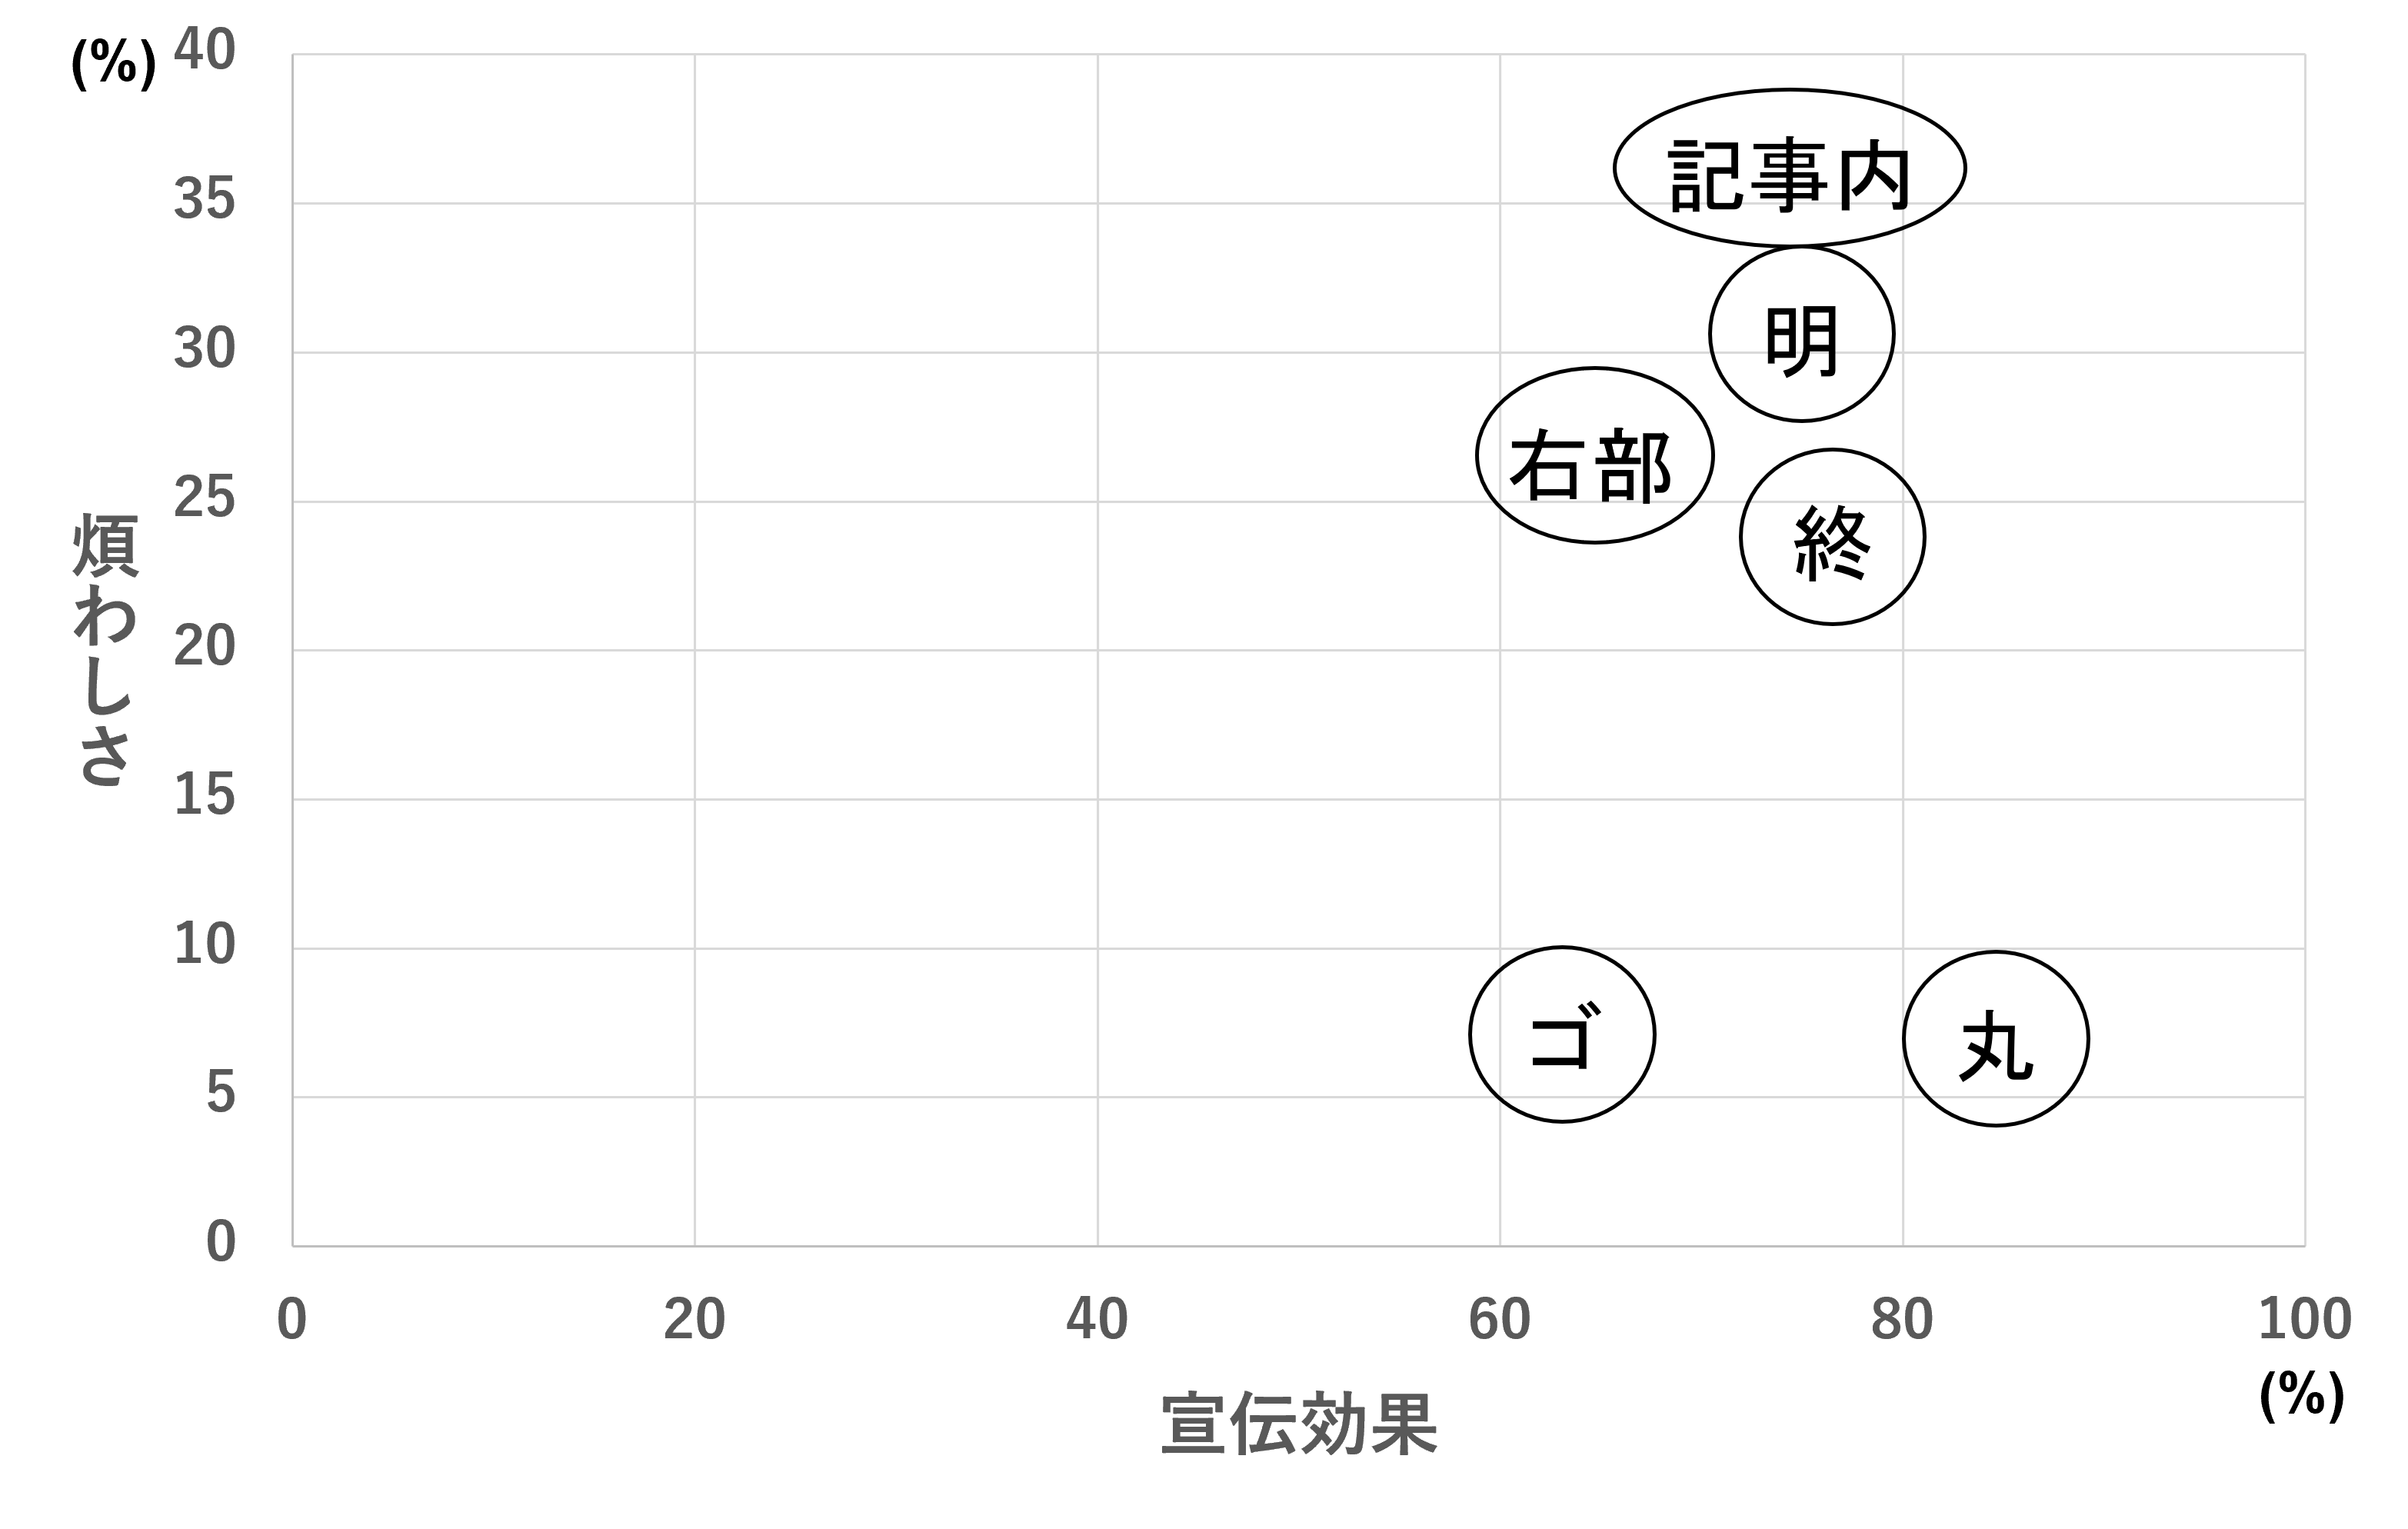
\includegraphics[height=45mm]{結果.png}
\end{center}
 \caption{広告配置とフォントを変化させた際の\\煩わしさと宣伝効果に関する調査結果}
 \label{fig:結果}
\end{figure}

\section{考察とまとめ}
本研究では,パソコン上のWebサイトの広告について,広告配置と広告のフォントの影響について調査を行った.
その結果,煩わしさと宣伝効果に相関がないことと,丸ゴシック体を使用した広告を記事終わりに配置することが適することが明らかになった.

\begin{thebibliography}{99}
\bibitem{mobile} 中島 弘貴,柗本 真佑,楠本 真二, ``モバイル端末におけるWeb広告の配置方法に対する一検討'', 信学技報, Vol.117, No.389, pp.69-74, 2018年
\bibitem{dentsu} 株式会社電通, ``2021年 日本の広告費'', \url{https://www.dentsu.co.jp/news/release/2022/0224-010496.html}, 2022/7/29参照
\end{thebibliography}

\end{document}
